%% ===================================================================
%%  Entrega v2 -- 2026-08-31
%%  Idea del proyecto + Marco teorico + Bibliografia -- Proyecto Wordglow
%%  Compilar:  pdflatex marco_teorico.tex   (dos veces)
%%  Requiere wordglow.cls y la carpeta image/ en esta misma ubicacion.
%% ===================================================================
\documentclass[letterpaper]{wordglow}

%% Fija figuras y tablas en el punto del texto donde se declaran (posicion [H]),
%% para que no floten a otra pagina dejando huecos grandes.
\usepackage{float}
%% No estirar el texto verticalmente para llenar la pagina.
\raggedbottom

\wgTitulo{IDEA Y MARCO\\\wgac{TE\'ORICO}}
\wgEyebrow{Taller de Grado I \textperiodcentered\ UMSS}
\wgKicker{Entrega v2}{Idea del proyecto, marco te\'orico y bibliograf\'ia}
\wgAutor{Adrian Andrade Medina}
\wgVersion{0.3 (borrador)}
\wgFecha{31/08/26}

\wgMarca{Wordglow}
\wgSubtitulo{Idea y marco te\'orico}
\wgWeb{UMSS \textemdash\ Ingenier\'ia Inform\'atica}
\wgCorreo{Taller de Grado I}
\wgTel{Gesti\'on 2026}
\wgDireccion{Cochabamba, Bolivia}

\begin{document}

\maketitle

\pagenumbering{roman}
\wgindice
\clearpage
\pagenumbering{arabic}

% ===================================================================
\wgchip{Parte 1}
\section{Idea del proyecto}

Aprender a leer en ingl\'es se atasca casi siempre en el mismo punto: no
alcanza el vocabulario. El lector se detiene en cada l\'inea, pierde el
hilo y termina abandonando. Las herramientas que existen tratan ese
problema por partes. Un lector interactivo traduce palabras al tocarlas
pero no programa un repaso serio; un gestor de flashcards repasa bien
pero deja al usuario la tarea de decidir y teclear qu\'e estudiar.

\textbf{Wordglow} es una aplicaci\'on m\'ovil que junta las dos mitades. Cada
d\'ia genera un cuento corto en ingl\'es, graduado por inteligencia
artificial al nivel de vocabulario del usuario y acompa\~nado de una
imagen y de lectura en voz alta. En el texto, cada palabra es
interactiva: al tocarla se abre su traducci\'on, su fon\'etica, su audio y
la oraci\'on donde aparece, y el usuario marca su estado \textemdash nuevo,
aprendiendo, dominado o ignorado\textemdash con un color de fondo.

La idea central es que \textbf{el mismo texto que se lee por gusto sea la
fuente del estudio deliberado}. Las palabras que el lector no domina se
convierten en tarjetas de repaso sin que \'el las escriba, y un algoritmo
de repetici\'on espaciada tipo SM-2 decide cu\'ando volver a mostrar cada
una, priorizando las que est\'an en aprendizaje y las vencidas del d\'ia.
Lectura y repaso dejan de ser actividades separadas: se alimentan entre
s\'i. Sobre esa base, una racha diaria y una pantalla de celebraci\'on
sostienen el h\'abito.

\subsection{Alcance}

El proyecto cubre la lectura y el vocabulario receptivo del ingl\'es en
una app solo m\'ovil, con progreso guardado en un backend y estado de
palabra global \textemdash el mismo para todos los cuentos\textemdash. Quedan
fuera la gram\'atica, la escritura, la producci\'on oral, la comprensi\'on
auditiva como destreza evaluada, otros idiomas y las certificaciones.

\subsection{Aporte y problema t\'ecnico abierto}

Ninguna herramienta actual re\'une en una sola pieza el cuento diario
generado con IA, el repaso espaciado con tarjetas sacadas del propio
texto y el acompa\~namiento con imagen y voz. Esa integraci\'on es el aporte
que persigue Wordglow. Trae adem\'as un problema t\'ecnico sin soluci\'on
est\'andar: el resaltado palabra por palabra durante la s\'intesis de voz en
m\'oviles, que conviene resolver con las marcas de tiempo del proveedor de
voz y no con temporizadores estimados.

% ===================================================================
\clearpage
\wgchip{Parte 2}
\section{Marco te\'orico}

Aprender a leer en ingl\'es depende de una cosa antes que de cualquier
otra: conocer suficientes palabras. Este cap\'itulo fija los conceptos que
sostienen la idea anterior y descarta lo que pertenece a la fase de
implementaci\'on (lenguajes, servicios, metodolog\'ia de desarrollo, dise\~no
de interfaz). Se apoya en cuatro fuentes: Nation (2013) y Schmitt (2008)
para la adquisici\'on de vocabulario, Roediger y Butler (2011) para el
papel de la memoria y Wo\'zniak y Gorzela\'nczyk (1994) para la repetici\'on
espaciada.

\subsection{Objeto de estudio}

El objeto de estudio es el aprendizaje de vocabulario receptivo del
idioma ingl\'es apoyado por una aplicaci\'on m\'ovil, donde la lectura de
textos breves y un mecanismo de repetici\'on espaciada forman el n\'ucleo
del proceso. Dentro de la Inform\'atica, el problema es de algoritmos y
t\'ecnicas de aprendizaje asistido por computadora, con un componente de
tecnolog\'ia emergente: el contenido de lectura lo genera un modelo de
inteligencia artificial.

\subsection{Aprendizaje de vocabulario en una lengua extranjera}

Conocer una palabra no es saber su traducci\'on. Nation (2013) lo
descompone en tres dimensiones \textemdash forma oral y escrita, significado
y uso\textemdash y sostiene que ese conocimiento se construye por grados, a
lo largo de muchos encuentros con la palabra en contexto. El proyecto se
centra en el vocabulario receptivo: las palabras que el lector reconoce y
entiende, aunque todav\'ia no sepa producirlas.

Cu\'anto vocabulario hace falta depende de para qu\'e. Nation (2013) lo
cuantifica en familias de palabras \textemdash una base y sus formas
derivadas\textemdash y lo asocia a la cobertura l\'exica, el porcentaje del
texto o del discurso que ese vocabulario permite entender (Tabla 1).

\begin{table}[H]
\caption{Vocabulario necesario para hablar y leer en ingl\'es seg\'un la meta de uso}
\vskip4pt
\noindent\small
\begin{tabular}{@{}L{2.9in}R{1.6in}R{1.6in}@{}}
\wgth{Meta de uso} & \wgth{Familias de palabras} & \wgth{Cobertura l\'exica}\\
\wgtoprule
Conversaci\'on cotidiana (comunicaci\'on oral b\'asica) & 2\,000--3\,000 & $\sim$95\,\% oral\\
\wgrowrule
Participar con comodidad en el discurso oral & 6\,000--7\,000 & $\sim$98\,\% oral\\
\wgrowrule
Empezar a leer textos aut\'enticos sencillos & 3\,000--4\,000 & $\sim$95\,\% escrito\\
\wgrowrule
Leer con autonom\'ia novelas y peri\'odicos sin apoyo & 8\,000--9\,000 & $\sim$98\,\% escrito\\
\wgrowrule
\end{tabular}
\par\normalsize\vskip4pt
\wgnotafig{Adaptado de Nation (2013). La comprensi\'on razonable empieza cerca
del 95\,\% de cobertura; la lectura fluida sin ayuda externa exige alrededor
del 98\,\%.}
\end{table}

La distancia entre 3\,000 y 9\,000 familias marca el terreno donde
trabaja Wordglow. Schmitt (2008) precisa c\'omo se recorre: la ense\~nanza
expl\'icita funciona, pero la retenci\'on se juega en los encuentros
repetidos y espaciados con la palabra en contextos con sentido. De ah\'i
la mec\'anica del proyecto: cada palabra que aparece en un cuento puede
reaparecer, en el momento programado, en una sesi\'on de repaso.

\subsection{Memoria y recuperaci\'on activa}

Releer algo no lo fija en la memoria; intentar recordarlo, s\'i. Roediger
y Butler (2011) llaman a esto efecto de prueba (\textit{testing effect}):
recuperar la informaci\'on desde la memoria produce una retenci\'on a largo
plazo mucho mayor que volver a leerla o reconocerla de forma pasiva. El
efecto crece cuando esos intentos se reparten en el tiempo en lugar de
amontonarse en una sola sesi\'on.

Una tarjeta de repaso con autoevaluaci\'on aplica ambos principios a la
vez. El aprendiz intenta recordar el significado antes de comprobarlo, y
el sistema decide cu\'ando repetir ese intento (Figura 1).

\begin{figure}[H]
\caption{Estructura de una tarjeta de repaso y su ciclo de recuperaci\'on activa}
\centering
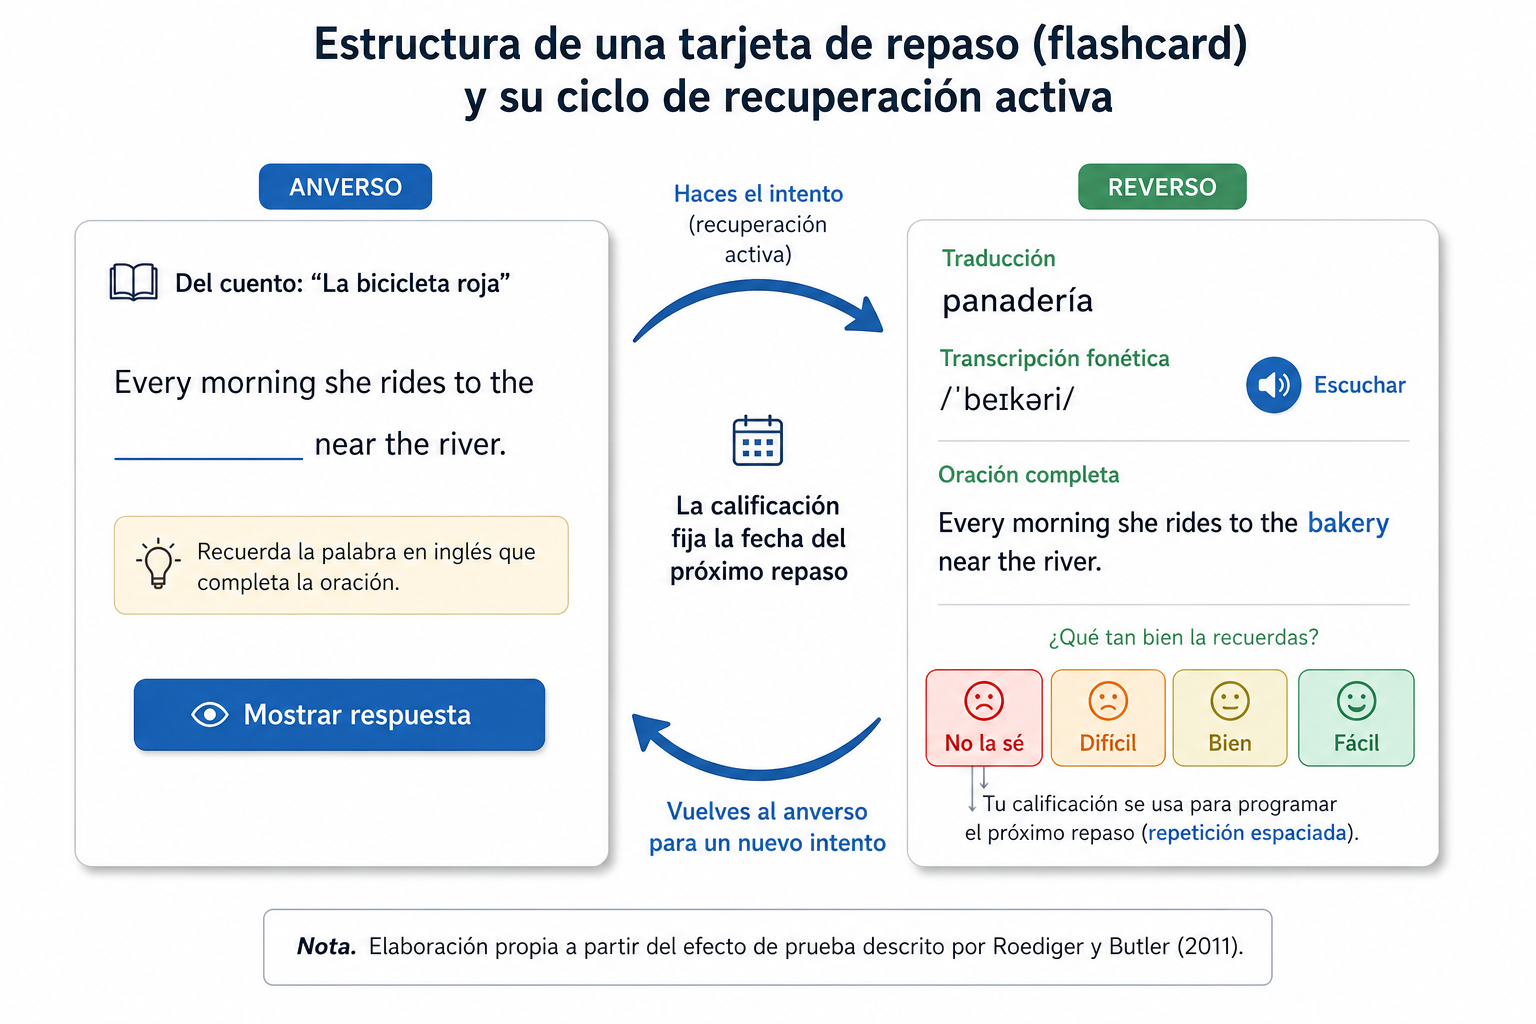
\includegraphics[width=\linewidth]{image/README/1788181670667.png}
\end{figure}

\subsection{Repetici\'on espaciada}

La repetici\'on espaciada programa cada repaso para el momento anterior al
olvido probable, con intervalos que se alargan a medida que la palabra se
afianza (Wo\'zniak y Gorzela\'nczyk, 1994). El objetivo es econ\'omico:
mantener la retenci\'on sobre un umbral con el menor n\'umero de repasos
posible (Figura 2).

\begin{figure}[H]
\caption{Retenci\'on de una palabra con repasos espaciados frente a un solo estudio}
\centering
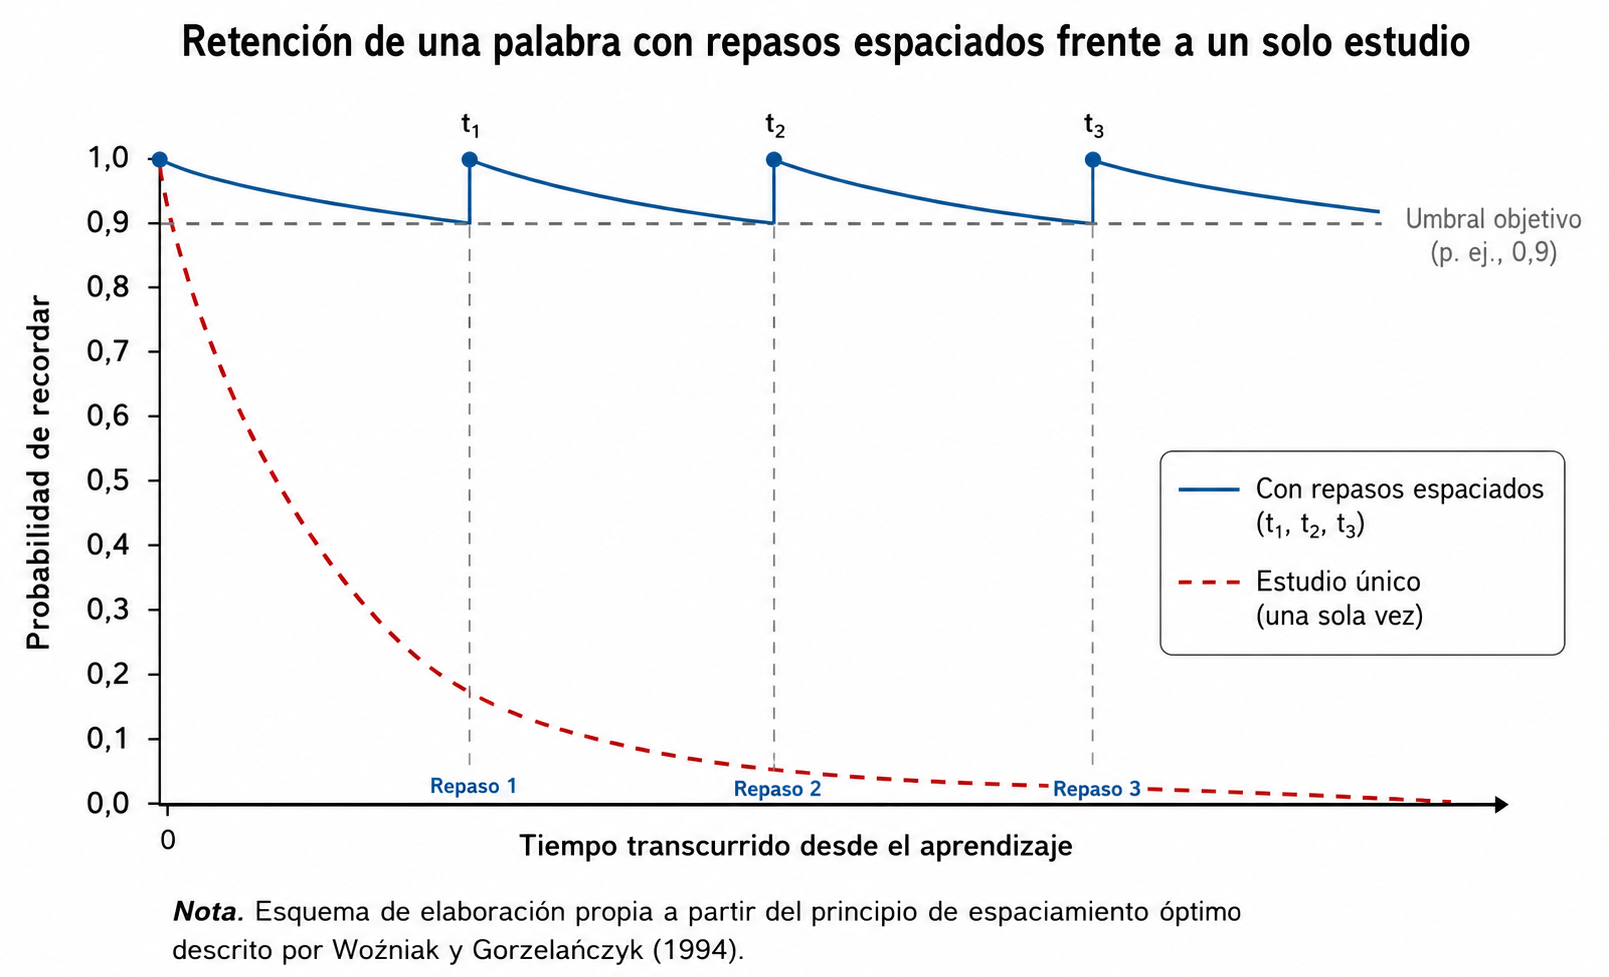
\includegraphics[width=\linewidth]{image/README/1788181499413.png}
\end{figure}

El algoritmo SM-2 de SuperMemo (Wo\'zniak y Gorzela\'nczyk, 1994) es la
implementaci\'on cl\'asica de esa idea. Cada tarjeta guarda un intervalo y
un factor de facilidad; tras cada respuesta, calificada de 0 a 5, el
intervalo se multiplica por el factor cuando el aprendiz acierta y se
reinicia cuando falla. Como los par\'ametros viven en la tarjeta, el
repaso se adapta a la dificultad de cada palabra y a cada usuario sin
necesidad de datos de terceros.

Wordglow parte de un repaso tipo SM-2 y a\~nade una regla de prioridad:
primero las palabras en estado ``aprendiendo'' y las vencidas del d\'ia.

\subsection{Estados de conocimiento de una palabra}

Si el conocimiento de una palabra es gradual (Nation, 2013), el sistema
necesita representarlo con m\'as de dos valores. Wordglow usa cuatro
estados, codificados por color sobre la palabra en el texto (Tabla 2).

\begin{table}[H]
\caption{Estados de conocimiento de una palabra en el modelo del proyecto}
\vskip4pt
\noindent\small
\begin{tabular}{@{}L{1.3in}L{2.5in}L{2.5in}@{}}
\wgth{Estado} & \wgth{Significado para el aprendiz} & \wgth{Tratamiento en la aplicaci\'on}\\
\wgtoprule
Nuevo & No ha sido vista ni marcada a\'un. & Se resalta; entra al repaso como \'item nuevo.\\
\wgrowrule
Aprendiendo & Reconocida con esfuerzo o con fallos recientes. & Se resalta; prioridad alta en el repaso.\\
\wgrowrule
Dominado & Reconocida de forma estable y autom\'atica. & Puede mostrarse sin resalte; repaso a intervalos largos.\\
\wgrowrule
Ignorado & Nombre propio, marca o top\'onimo. & Sin resalte; excluida de m\'etricas y de repaso.\\
\wgrowrule
\end{tabular}
\par\normalsize\vskip4pt
\wgnotafig{El estado es global: vale para todas las apariciones de la palabra
en cualquier cuento, no para un cuento concreto.}
\end{table}

\subsection{Estado del arte}

Los tres pilares de Wordglow tienen respaldo por separado. En
vocabulario, Nation (2013) y Schmitt (2008) coinciden en que el
aprendizaje exige encuentros repetidos y espaciados en contextos con
significado. En memoria, Roediger y Butler (2011) sit\'uan la recuperaci\'on
activa y distribuida como el mecanismo que fija lo aprendido. En
algoritmos, el SM-2 de Wo\'zniak y Gorzela\'nczyk (1994) sigue siendo la
referencia para programar esos repasos por \'item.

Las herramientas actuales cubren piezas sueltas. Duolingo aplica
repetici\'on espaciada sobre contenido fijo; Anki lo hace sobre tarjetas
que crea el usuario, sin texto de lectura; LingQ y Readlang ofrecen
lectura con palabras interactivas y traducci\'on al tocar, pero con un
repaso limitado. Ninguna re\'une en una sola herramienta el cuento diario
generado y graduado con IA, el repaso espaciado cuyas tarjetas salen del
propio texto le\'ido y el acompa\~namiento con imagen y lectura en voz alta
con seguimiento visual. Ese vac\'io es la contribuci\'on que persigue el
proyecto.

% ===================================================================
\clearpage
\wgchip{Parte 3}

%% El entorno "referencias" del formato rotula "Referencias"; esta entrega
%% lo presenta como "Bibliograf\'ia" sin cambiar la clase compartida.
\makeatletter
\renewenvironment{referencias}
  {\section*{Bibliograf\'ia}\addcontentsline{toc}{section}{Bibliograf\'ia}%
   \vskip15pt
   \begingroup\fontsize{9.75}{19.5}\selectfont\setlength{\parskip}{0pt}}
  {\endgroup\par}
\makeatother

\begin{referencias}
\refitem Nation, I.~S.~P. (2013). \textit{Learning vocabulary in another
language} (2.\textsuperscript{a} ed.). Cambridge University Press.
\refitem Roediger, H.~L. y Butler, A.~C. (2011). The critical role of
retrieval practice in long-term retention. \textit{Trends in Cognitive
Sciences, 15}(1), 20--27. https://doi.org/10.1016/j.tics.2010.09.003
\refitem Schmitt, N. (2008). Instructed second language vocabulary
learning. \textit{Language Teaching Research, 12}(3), 329--363.
https://doi.org/10.1177/1362168808089921
\refitem Wo\'zniak, P.~A. y Gorzela\'nczyk, E.~J. (1994). Optimization of
repetition spacing in the practice of learning. \textit{Acta
Neurobiologiae Experimentalis, 54}(1), 59--62.
\end{referencias}

\wgcierre

\end{document}
